\section{Which Memories Become Useful Evidence?}
\label{sec:memory-use}

Memory questions impose requirements on information that simple topical relevance does not specify: a changed relationship determines which further evidence is needed; a historical question refers to an earlier event; and a speaker or date restricts which otherwise accurate statement can answer the question.
We study how AMOR's context recommendation and presentation respond to these requirements.
The analysis covers four data origins: document QA from RULER, MQuAKE-derived FactConsolidation (FC), LoCoMo conversations, and 2WikiMultiHopQA.
We retain all six evaluation settings and their full released configurations: 100 questions per document/FC setting, all 1,986 LoCoMo questions, and the 1,000-question 2Wiki release used by HippoRAG~2.
All answer comparisons use the original metrics and four readers; this is the same seed-42 development evaluation as the main experiments.
The graph comparisons freeze recognition, initial scores, source texts, damping, rank fusion, and the five-source budget.

\subsection{Selecting Further Evidence, Beyond Confirming a Match}
\label{sec:memory-evidence}

\paragraph{A relation can identify where to look without supplying what to read.}
In 2Wiki, HippoRAG~2 finds at least one annotated support passage for all 1,000 questions, but finds all support passages for only 469; AMOR reaches 689.
The effect depends on the question's dependency structure: among questions with two support passages, complete support rises from 44.1\% to 72.4\% for \emph{compositional} questions, but only from 94.3\% to 96.3\% for \emph{comparison} questions.
This motivates a more specific test than whether graph propagation beats matching: does the construction recommend useful additional sources once the relevant facts are already recognized?

CatRAG already addresses incomplete evidence and introduces a query-specific key-fact edge boost~\citep{lau-etal-2026-breaking}.
We therefore compare this published operation on the \emph{same} entity--source graph, rather than attributing an entire system difference to graph recommendation.
The released operator multiplies the forward links supported by recognized facts by 2.5 and renormalizes each entity's passage-edge mass; a separate condition follows the paper's $1+\beta$ rule with $\beta=2.5$.
Reciprocal directed arcs reproduce AMOR's original unmodified scores and selections before either intervention.
Figure~\ref{fig:memory-operations} compares these controls with unit weights and AMOR's fixed weights, which accumulate the contributions of all retained facts.
On all 1,000 2Wiki questions, the recognized-fact boost changes complete support from 63.5\% to 63.7\% on unit weights (seven gains, five losses).
AMOR reaches 68.9\%, with 54 gains and two losses relative to boosted unit weights; adding the boost to AMOR reaches 69.4\% (six gains, one loss).
Following the paper's $1+\beta$ rule instead gives 63.5\% and 69.5\%, respectively.


The preselected film example in Table~\ref{tab:memory-examples} makes the changed recommendation concrete.
Both films and their directors have already been recognized; the missing text is a director's biography needed for the age comparison.
Lowering just its entity--biography weight from 26 to 1 removes that biography from the five selected sources; restoring this edge's weight on the unit graph adds it back.
The accepted facts and other weights remain fixed.
The weight comes from 50 retained triples about this entity in that source, plus the base connection; it does not encode the answer or a newly discovered reasoning path.

\paragraph{The same distinction matters when relationships change.}
MQuAKE already establishes the difficulty of using edits in subsequent reasoning~\citep{zhong-etal-2023-mquake}; here we locate the failure in the \emph{selection of further text}.
In the FC-MH example, both HippoRAG~2 and AMOR without recommendation supply the synthetic update making George Eliot the author of \emph{Dubliners}, yet omit her death-location source.
AMOR recommends that source second.
Replacing only the accepted authorship with the actual older extracted relation removes the death source and makes all four readers incorrect, although the corrected authorship remains in their input; restoration recovers all four answers.
On all 100 FC-MH questions, expanding recognition to all extracted facts while retaining the same graph lowers EM from 14/16/10/6 to 11/12/9/3.
The population result is modest in absolute accuracy, but the intervention distinguishes supplying a correction from using it to select its consequences.

\begin{figure*}[t]
\centering
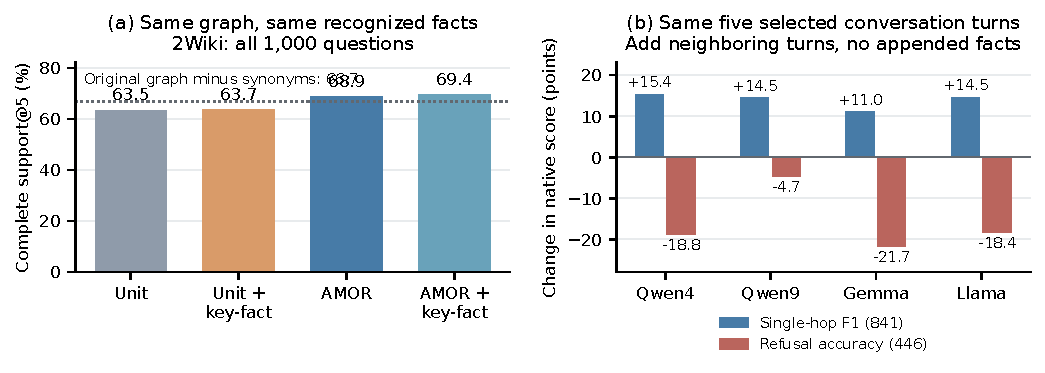
\includegraphics[width=\textwidth]{figures/memory_operations.pdf}
\caption{\textbf{Controlled changes in memory use.} (a) All 1,000 2Wiki questions, with identical graph connections, recognized facts, initial scores, and five-source budget. Key-fact conditions apply CatRAG's operator to the unit graph; they are not the full CatRAG system. The dotted line is the separate original-graph control with synonym edges removed. (b) Adding neighboring conversation turns to the same five selected turns improves single-hop F1 but reduces refusal accuracy. No appended facts are present in either condition. Each reader is shown separately.}
\label{fig:memory-operations}
\end{figure*}

\subsection{What Consolidation Removes Can Reappear at Answer Time}
\label{sec:memory-presentation}

\paragraph{Selection and presentation can disagree about the active assertion.}
AMOR's retained facts govern graph construction and candidate selection, while original source text remains available.
In FC-SH, both the obsolete USA assertion and the newer UK assertion about \emph{Witches of East End} enter the selected text, even though only the UK fact survives consolidation.
Ranking the updated source first is insufficient: without appended facts, none of the four readers receives native credit.
Appending the retained UK assertion makes all four correct.
Removing only that assertion, with the five texts and nine other appended facts fixed, reverses all four scores; replacing it with the extracted USA assertion also fails, and restoration recovers them.

This effect extends beyond the example.
On all 100 FC-SH questions, changing augmentation candidates from retained to all extracted facts reduces EM by 15/14/15/17 points, at the same five-source and ten-fact budgets.
For comparison, the recognition-candidate intervention on FC-MH costs 3/4/1/3 points.
These operations act at different stages: current associations determine which further sources are recommended, while the selected assertions affect how competing original texts are used.
The large presentation effect prevents attributing FC-SH's improvement solely to graph construction.

\paragraph{The benefit is conditional on what the question asks memory to preserve.}
LoCoMo exposes the opposite need: a past event must remain answerable even after a later event uses the same relation.
LightMem already identifies mistaken consolidation as a source of information loss~\citep{fang2026lightmem}; our trace follows that loss through selection and recovery.
For Nate's activity during Joanna's road trip, OpenIE correctly extracted the fourth video-game-tournament win, but AMOR's later-source selection removed it after another \emph{won} statement.
The annotated reply is still ranked first, yet says only ``while you were winning.''
Its neighboring original turn supplies the missing event.
Removing that turn reduces native F1 from 80/80/75/80 to 0/0/0/40; restoring the original extracted fact to the five central turns gives 80/88.9/100/100.
Thus the source context compensates for a loss introduced by AMOR's own construction, rather than merely repeating its retained facts.

Across LoCoMo's answerable categories, 104 of 2,345 resolvable question/annotated-turn occurrences have all their extracted facts removed and become isolated in the graph.
The selected central turns contain 23 of these occurrences; adding their fixed neighbors includes 55.
The all-question context experiment in Figure~\ref{fig:memory-operations} shows that neighboring text improves the 841 single-hop questions more than appending the selected facts alone.
Preserving source history is therefore useful even when the memory already stores compact facts, but its benefit comes from information that fact selection did not preserve.

\begin{table*}[t]
\centering
\small
\setlength{\tabcolsep}{4pt}
\begin{tabular}{p{.18\textwidth}p{.31\textwidth}p{.30\textwidth}p{.16\textwidth}}
\toprule
Question / source & Verified information in the source & Change in supplied evidence & Observed outcome \\
\midrule
Older film director?\newline 2Wiki & \emph{God's Gift to Women}: Michael Curtiz; Curtiz born 1886; Edith Carlmar born 1911. & Lower only Curtiz--biography weight $26\to1$; restore $1\to26$ on unit graph. & Complete support $4/4\to3/4$; restoration gives $4/4$. \\
\addlinespace[3pt]
Death place of \emph{Dubliners}' author?\newline FC-MH & Update 7516 names George Eliot; statement 13652 gives London. & Substitute older accepted authorship. Update remains in input; London source disappears. & Native-correct readers $4/4\to0/4\to4/4$ after restoration. \\
\addlinespace[3pt]
Country of \emph{Witches of East End}?\newline FC-SH & Old statement 1836: USA; later statement 4787: UK. Both texts are selected. & Remove only appended UK assertion; keep all five texts and other nine facts. & Native-correct readers $4/4\to0/4\to4/4$ after restoration. \\
\addlinespace[3pt]
Kirton End's city population in 2001?\newline MH-Doc & Distractor: a different Kirton, 1,146 in 2011. Correct source: Boston town, 35,124 in 2001. & AMOR supplies the Boston source and dated fact; HippoRAG~2 supplies the Kirton distractor. & AMOR $4/4$; seven external baselines each $0/4$. \\
\addlinespace[3pt]
Nate's activity during Joanna's trip?\newline LoCoMo & D17:2: ``while you were winning''; D17:1 identifies the fourth video-game-tournament win. & Remove the explanatory neighboring turn from otherwise unchanged full context. & F1: $80/80/75/80\to0/0/0/40$. \\
\addlinespace[3pt]
Melanie's art-show inspiration?\newline LoCoMo & D9:16 describes \emph{Caroline}'s inspiration: visiting an LGBTQ center. & Add neighboring turns and facts to the five central turns; all readers adopt the wrong speaker's event. & Correct refusals $4/4\to0/4$. \\
\bottomrule
\end{tabular}
\caption{\textbf{Examples with source checks and local interventions.} Four-reader scores follow Qwen4/Qwen9/Gemma/Llama order. FC updates are benchmark counterfactuals. The 2Wiki fractions count annotated support passages, not readers. MH-Doc is a system comparison; the other interventions keep the components stated in the table fixed. Full texts, native predictions, and all adverse outcomes accompany the analysis.}
\label{tab:memory-examples}
\end{table*}

\subsection{More Relevant Context Can Cross the Wrong Boundary}
\label{sec:memory-boundaries}

The neighboring turns that recover historical details also create a measurable cost.
With the five central turns fixed and no appended facts, adding neighbors improves single-hop F1 by 15.40/14.48/11.04/14.51 points, but lowers refusal accuracy on all 446 adversarial questions by 18.83/4.71/21.75/18.39 points.
LoCoMo already discusses speaker misattribution~\citep{maharana-etal-2024-evaluating}; this control identifies the same source-expansion operation as both a benefit and a liability.
In the Melanie example, all readers initially refuse correctly and all four fail with full context.
Removing Caroline's explanation restores refusal for three readers; the fourth remains incorrect under every single-turn removal.
The original text contains the correct speaker identity, so the failure is not explained by a missing name alone.

The documentary case shows an analogous qualification problem outside dialogue: the retrieved population statement concerns the wrong town and year.
Across all 100 MH-Doc questions, recommendation corrects 18/16/15/21 answers and introduces 5/3/6/6 errors relative to the matching-based control, yielding net gains of 13/13/9/15 EM points.
On SH-Doc the corresponding gains are 9/11/10/8 points; in contrast, recommendation slightly reduces overall LoCoMo scores for the two Qwen readers.
The task matters: finding related material helps when it supplies the missing documentary association, while additional related conversation can encourage an answer that the requested speaker's history does not support.

Together, the experiments explain distinct contributions to AMOR's performance: constructing useful associations affects which complementary sources enter the context; retained assertions affect the use of conflicting text; preserved source history recovers information discarded during construction.
Recommendation makes additional evidence available, but the relevant relationship, historical event, speaker, and date determine whether that evidence answers the question.
